%http://www.math.uconn.edu/~kconrad/blurbs/
\documentclass[oneside,a4paper,12pt]{article}
\usepackage[english,brazilian]{babel}
\usepackage[alf]{abntex2cite}
\usepackage[utf8]{inputenc}
\usepackage[T1]{fontenc}
\usepackage[top=20mm, bottom=20mm, left=20mm, right=20mm]{geometry}
\usepackage{framed}
\usepackage{booktabs}
\usepackage{color}
\usepackage{hyperref}
\usepackage{graphicx}
\usepackage{float}
\usepackage{pstricks}
\graphicspath{{./Figuras/}}    
\definecolor{shadecolor}{rgb}{0.8,0.8,0.8}
\usepackage{textcomp}
\usepackage{tikz}
\usepackage[utf8]{inputenc}
\usepackage{mathtext}
\usepackage{graphicx}
\usepackage{verbatim}
\usepackage{wrapfig}
\usepackage[T1]{fontenc}
\usepackage{blindtext}
\usepackage{tasks}
\usepackage{fancybox}
\usepackage{amsthm}
\usepackage{setspace}
\usepackage{amsmath}
\usepackage{amsfonts}
\usepackage{amssymb}
\usepackage{graphicx, color}
\newcommand{\under}{\texttt{\char`_}}
\newcommand{\sen}{{\rm sen}}
\newcommand{\tg}{{\rm tg}}
\newcommand{\cotg}{{\rm cotg}}
\newcommand{\cossec}{{\rm cossec}}
\newcommand{\arctg}{{\rm arctg}}
\newcommand{\arcsen}{{\rm arcsen}}
\newcommand{\negrito}[1]{\mbox{\boldmath{$#1$}}} 
\usepackage{pifont}
\usepackage{multicol}
\usepackage[framemethod=TikZ]{mdframed}
\newcommand{\heart}{\ensuremath\heartsuit}
\newcommand{\diamonde}{\ensuremath\diamondsuit}
\theoremstyle{Colorido}
\newtheorem{questao}{\textcolor{Floresta}{\textit{\bf Questão}}}
\newtheoremstyle{Colorido}{}{}{\color{Floresta}}{}{\color{Floresta}\bfseries}{}{ }{}
\newtheorem{theorem}{Theorem}
\newtheoremstyle{solu}{}{}{}{}{\color{red}\bfseries}{}{ }{}
\theoremstyle{solu}
\newtheorem*{resp}{Solução}
\newtheoremstyle{dotlessP}{}{}{}{}{\color{Floresta}\bfseries}{}{ }{}
\theoremstyle{dotlessP}
\newcommand{\solucao}[1]{\textcolor{blue}{\textbf{Solução:} #1}}
\newtheorem{sol}{Questão}
%FAZ EDICOES AQUI (somente no conteudo que esta entre entre as ultimas  chaves de cada linha!!!)
\newcommand{\universidade}{Programa de Iniciação Científica OBMEP}
\newcommand{\centro}{PIC 2020}
%\newcommand{\departamento}{Departamento}
%\newcommand{\curso}{Curso}
\newcommand{\professor}{Douglas de Araujo Smigly}
\newcommand{\disciplina}{Programa de Iniciação Científica}
\newcommand{\entrega}{ }
\DeclareSymbolFont{extraup}{U}{zavm}{m}{n}
\DeclareMathSymbol{\varheart}{\mathalpha}{extraup}{86}
\DeclareMathSymbol{\vardiamond}{\mathalpha}{extraup}{87}
	\cornersize{.3} 
	\mdfdefinestyle{MyFrame}{%
    linecolor=blue,
    outerlinewidth=2pt,
    roundcorner=20pt,
    innertopmargin=\baselineskip,
    innerbottommargin=\baselineskip,
    innerrightmargin=20pt,
    innerleftmargin=20pt,
    backgroundcolor=gray!24!white}
%ATE AQUI !!!

\begin{document}
\definecolor{Floresta}{rgb}{0.13,0.54,0.13}
	\pagestyle{empty}
	
	\begin{center}
	
\includegraphics[width=\linewidth/3]{logo_pic}%LOGOTIPO DA INSTITUICAO
	 	\vspace{0pt}
	 	
		\universidade
		\par
		\centro
		\par
%		\departamento
		\par
%		\curso
		\par
		\vspace{24pt}
		\LARGE \textbf{Avalia\c c\~ao - Ciclo II}
		
	\end{center}
	
	\vspace{24pt}
	
	%
%	\begin{tabular}{ |l|p{12cm}| }
%		
%		\hline
%		\multicolumn{2}{|c|}{\textbf{Dados de Identificação}} \\
%			\hline
%		Disciplina:        &    \disciplina          \\
%		\hline
%		Professor:         &    \professor           \\
%	\hline
%	Aluno(a):         &\\
%		\hline
%	Multiplicidade:  & \ \ \ \ \ \ \vline Nível: \vline\\
%	
%		\hline
	%\end{tabular}
	%
	

	\begin{tabular}{ |l|p{12cm}| }
		
		\hline
		\multicolumn{2}{|c|}{\textbf{Dados de Identificação}} \\
			\hline
		Curso:        &  \disciplina \\
			\hline
		Nome:        &  \\
		\hline
		Nível:      &  \\
		\hline
				Multiplicidade:      &  \\
		\hline
				Assinatura:      &  \\
		\hline
				Data de entrega:      &  \entrega \\
		\hline
	\end{tabular}
	
	\vspace{24pt}
	\vspace{40pt}
	\tableofcontents
	\begin{comment}	
\begin{multicols*}{2}
	\begin{center}
		\begin{tabular}{ |c|p{1.9cm}| }
		
		\hline
		\multicolumn{2}{|c|}{\textbf{Tarefa Online}} \\
			\hline
		\centering\textbf{Questão}        &  \textbf{Resposta}\\
		\hline
		Questão 1        & (b)\\
		\hline
		Questão 2        & (c)\\
		\hline
		Questão 3        & (c)\\
		\hline
		Questão 4        &\\
		\hline
		Questão 5        &\\
		\hline
		Questão 6        &\\
		\hline
		\textbf{Total}        &\\
		\hline
	\end{tabular}
	\end{center}
\columnbreak
		\begin{center}
		\begin{tabular}{ |c|p{1.9cm}| }
		
		\hline
		\multicolumn{2}{|c|}{\textbf{Avaliação Online}} \\
			\hline
		\centering\textbf{Questão}        &  \textbf{Resposta}\\
		\hline
		Questão 1        &\\
		\hline
		Questão 2        &\\
		\hline

		\textbf{Total}        &\\
		\hline
	\end{tabular}
	\end{center}
	
	\end{multicols*}
	\vspace{24pt}
	\end{comment}
	%\begin{snugshade}
	%	\section{O... aumento  }  
	%\end{snugshade}
	\newpage	
	\textcolor{Floresta}{\section{Tarefa Online}}
	\begin{sol}
\textit{(0,5 ponto)} 
Uma fila de cinema tem $10$ cadeiras, nas quais devem se sentar $7$ adultos e $3$ crianças. O número de maneiras que isso pode ser feito se quaisquer  crianças não devem ficar em cadeiras contíguas é igual a:
\begin{tasks}[counter-format={(tsk[a])},label-width=3.6ex, label-format = {\bfseries}, column-sep = {20pt}](5)
\task[\textcolor{blue}{$\negrito{(a)} $}] $1693440$
\task[\textcolor{blue}{$\negrito{(b)} $}] $1753250$ 
\task[\textcolor{blue}{$\negrito{(c)} $}] $1847540$
\task[\textcolor{blue}{$\negrito{(d)} $}] $1942980$
\task[\textcolor{blue}{$\negrito{(e)} $}] $2043850$
\end{tasks}
\end{sol}
\solucao{O número de modos de arrumar os $7$ adultos em fila é igual a $7!=5040$. Se $A_1$, $A_2$, $A_3$, $A_4$, $A_5$, $A_6$ e $A_7$ denotam os $7$ adultos, uma das possíveis arrumações é, por exemplo\[\under  \ A_1 \ \under \  A_3 \ \under \ A_5 \ \under \ A_2 \ \under \ A_4 \ \under \ A_7 \ \under \ A_6 \ \under \] Agora, temos que colocar as crianças nos $8$ espaços ($\under$) acima. Como em nenhum espaço podem ficar duas crianças, ocuparemos $3$ espaços (com uma criança em cada) e deixaremos $5$ espaços vazios. O número de maneiras de escolher os espaços que ocuparemos é igual a $C_8^3=56$. Uma vez escolhidos os três espaços que as crianças ocuparão, é preciso observar que há $3!=6$ maneiras de dispor as crianças nesses espaços, Assim, pelo Princípio Multiplicativo, a resposta é $5040\times56\times6=1693440$.}
		%\vspace{60pt}
		\newpage	
	\begin{sol}
\textit{(0,5 ponto)} \newline \newline
O número de maneiras de colorir $6$ objetos com $3$ cores, sendo que cada objeto deve ser colorido com uma única cor e cada cor tem que ser usada pelo menos uma vez, é igual a:
\begin{tasks}[counter-format={(tsk[a])},label-width=3.6ex, label-format = {\bfseries}, column-sep = {20pt}](5)
\task[\textcolor{blue}{$\negrito{(a)} $}] $452$
\task[\textcolor{blue}{$\negrito{(b)} $}] $473$
\task[\textcolor{blue}{$\negrito{(c)} $}] $498$      
\task[\textcolor{blue}{$\negrito{(d)} $}] $524$
\task[\textcolor{blue}{$\negrito{(e)} $}] $540$
\end{tasks}
\end{sol}
\textcolor{blue}{O número de maneiras de colorir os $6$ objetos com as $3$ cores, sem restrições, é igual a $3^6=729$, uma vez que há $3$ cores que podem ser escolhidas para cada um dos $6$ objetos. Porém, nessa contagem estão incluídas colorações dos $6$ objetos sem usar uma das três cores e, portanto, devemos excluir essas colorações. Há $C_3^2 = \binom{3}{2} =3$ maneiras de escolher $2$ cores, dentre as $3$ cores, para colorir os objetos. Uma vez escolhidas $2$ cores, o número de maneiras de colorir os $6$ objetos com essas $2$ cores é igual a $2^6=64$. Assim, o número de maneiras de colorir os $6$ objetos com $2$ cores, dentre as $3$ cores, é igual a $3\cdot64=192$. Assim, aparentemente a resposta seria $729-192=537$. Porém, quando subtraímos $192$ descontamos duas vezes as colorações dos objetos com uma única cor (por exemplo, supondo que as $3$ cores sejam branco, azul e verde, ao escolhermos $\{\mbox{branco}, \mbox{azul}\}$, no total das $64$ colorações com essas duas cores foi contada a coloração com todos os objetos coloridos de branco, e ao escolhermos $\{\mbox{branco}, \mbox{verde}\}$, no total das $64$ colorações com essas duas cores também foi contada a coloração com todos os objetos coloridos de branco). Assim, na contagem de $537$, devemos incluir as colorações dos $6$ objetos com uma única cor, que é um total de $3$ colorações. Assim, a resposta final é $537+3=540$.}
\newpage
	\begin{sol}
\textit{(0,5 ponto)} \newline \newline Em um congresso há $5$ professores de Matemática e $5$ professores de Física. Deve-se formar uma comissão de $4$ professores e os mesmos são escolhidos ao acaso dentre os $10$ professores. A probabilidade de a comissão ser formada por exatamente $2$ professores de Matemática e $2$ professores de Física é:

\begin{tasks}[counter-format={(tsk[a])},label-width=3.6ex, label-format = {\bfseries}, column-sep = {20pt}](5)
\task[\textcolor{blue}{$\negrito{(a)} $}] $\dfrac{2}{21}$
\task[\textcolor{blue}{$\negrito{(b)} $}] $\dfrac{5}{21}$
\task[\textcolor{blue}{$\negrito{(c)} $}] $\dfrac{10}{21}$
\task[\textcolor{blue}{$\negrito{(d)} $}] $\dfrac{13}{21}$
\task[\textcolor{blue}{$\negrito{(e)} $}] $\dfrac{20}{21}$
\end{tasks}
\end{sol}
\solucao{Dos $10$ professores, podemos escolher $4$ professores de $C_{10}^4 = \binom{10}{4}$ formas. Podemos escolher exatamente $2$ professores de Matemática e $2$ professores de Física de $C_5^2 \times C_5^2 = \binom{5}{2} \times \binom{5}{2}$ formas.Logo, a probabilidade procurada é\[\dfrac{C_5^2 \times C_5^2}{C_{10}^4}=\dfrac{\frac{5\times 4}{2} \times \frac{5\times 4}{2}}{\frac{10\times 9\times 8 \times 7}{1\times 2 \times 3 \times 4}} = \dfrac{5 \times 2 \times 5 \times 2 \times 2 \times 3 \times 4}{10\times 9\times 8 \times 7} =\dfrac{10}{21}\]Logo, a alternativa correta é a (c).}
\newpage
	\begin{sol}
\textit{(0,5 ponto)} \newline \newline A figura abaixo representa o mapa de uma cidade, na qual há $7$ avenidas na direção norte-sul e $6$ avenidas na direção leste-oeste.
\begin{center}
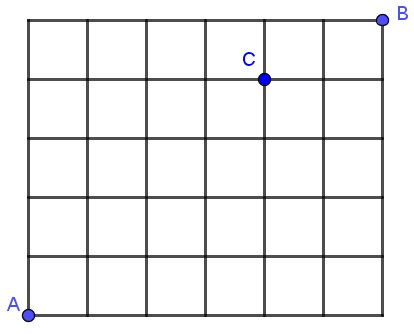
\includegraphics[scale=0.7]{Provas e Avaliações/arq-01ciclo2.jpg}    
\end{center}

Todo dia Marcos parte de sua casa, que se encontra no ponto $A$, e se dirije para a escola, no ponto $B$. Em cada cruzamento de avenidas, Marcos escolhe ao acaso a direção que irá seguir, mas sempre de tal forma que o trajeto percorrido de sua casa até a escola seja de comprimento mínimo. A probabilidade de o trajeto percorrido por Marcos passe pela casa de seu amigo Fernando, que se encontra no ponto $C$, é:
\begin{tasks}[counter-format={(tsk[a])},label-width=3.6ex, label-format = {\bfseries}, column-sep = {20pt}](5)
\task[\textcolor{blue}{$\negrito{(a)} $}] $\dfrac{2}{33}$
\task[\textcolor{blue}{$\negrito{(b)} $}] $\dfrac{4}{33}$
\task[\textcolor{blue}{$\negrito{(c)} $}] $\dfrac{3}{22}$
\task[\textcolor{blue}{$\negrito{(d)} $}] $\dfrac{5}{11}$
\task[\textcolor{blue}{$\negrito{(e)} $}] $\dfrac{6}{11}$
\end{tasks}
\end{sol}
\solucao{Para que o trajeto de Marcos tenha comprimento mínimo, ele deve se dirigir sempre para o norte $(N)$ ou para o leste $(E)$. Se, em uma esquina dada, Marcos decide se dirigir para o norte, escreveremos $N$, e se decide se dirigir para o leste, escreveremos $E$. Dessa forma, cada trajeto de Marcos pode ser codificado como uma sequência de $N$'s e $E$'s. Pela figura, vemos que um trajeto que começa no ponto $A$ e termina no ponto $B$ deve estar formado por uma sequência de $5$ letras $N$ e $6$ letras $E$. Trata-se então de uma permutação de $11$ letras com elementos repetidos. Assim, o número de trajetos possíveis é $\dfrac{11!}{5! \cdot 6!}=462$. \\ Pelo Princípio Multiplicativo, para contar o número de trajetos que passam por $C$, devemos multiplicar o número de trajetos de $A$ até $C$ pelo número de trajetos de $C$ até $B$. Pela figura, um trajeto de $A$ até $C$ é codificado por uma sequência de $4$ letras $N$ e $4$ letras $E$ e um trajeto de $C$ até $B$ é codificado por uma sequência de $1$ letras $N$ e $2$ letras $E$. Dessa forma, o número de trajetos que passam por $C$ é $\dfrac{8!}{4! \cdot 4!} \cdot \dfrac{3!}{2! \cdot 1!}=210$. Assim, a probabilidade pedida é $\dfrac{210}{462}=\dfrac{5}{11}$.}
\newpage
	\begin{sol}
\textit{(4 pontos)} \newline \newline
Há $n$ livros em uma prateleira. De quantas maneiras os livros podem ser arrumados em ordens diferentes de modo que nenhum deles permaneça em seu lugar original,
\begin{tasks}[counter-format={(tsk[a])},label-width=3.6ex, label-format = {\bfseries}, column-sep = {20pt}](1)
\task[\textcolor{blue}{$\negrito{(a)} $}] se $n = 3?$
\task[\textcolor{blue}{$\negrito{(b)} $}] se $n = 4?$
\task[\textcolor{blue}{$\negrito{(c)} $}] se $n = 5?$
\end{tasks}
\end{sol}
\solucao{\textbf{Primeira Solução:}\begin{tasks}[counter-format={(tsk[a])},label-width=3.6ex, label-format = {\bfseries}, column-sep = {20pt}](1)\task[\textcolor{blue}{$\negrito{(a)} $}] Numere os livros 1, 2 e 3. Inicialmente, eles estão ordenados como 1, 2, 3 na prateleira. Se colocarmos o livro 1 na posição $2$, o livro 3 tem que ir para a posição $1$, de modo que o único resultado possível é 3, 1, 2. Se colocarmos o livro 1 na posição $3$, o livro 2 tem que ir para a posição $1$, de modo que o único resultado possível é 2, 3, 1. Logo, só há $2$ maneiras de arrumar os livros de modo que nenhum deles fique em sua posição original.\task[\textcolor{blue}{$\negrito{(b)} $}] Numere os livros 1, 2, 3 e 4. Inicialmente, eles estão ordenados como 1, 2, 3, 4 na prateleira. Podemos colocar o livro 1 na posição $2$, $3$ ou $4$. Com cada um desses movimentos, encontraremos o mesmo número de opções para arrumar os livros. Vamos contar, então, o número de arrumações possíveis quando o livro 1 fica na posição $4$ e depois multiplicar esse número por $3$, para obter o número total de arrumações possíveis. Coloque o livro 4 temporariamente na posição $1$, de modo que os livros fiquem ordenados como 4, 2, 3, 1. As duas arrumações possíveis (pelo item (a)) dos três primeiros livros (4, 2, 3, no momento) que não deixam nenhum em sua posição original irão dar arrumações dos quatro livros que não deixam nenhum em sua posição original. Além disso, a ordem 4, 3, 2 também é uma arrumação de 4, 2, 3 que muda a posição original dos quatro livros. Logo, existem $2+1=3$ arrumações possíveis de 4, 2, 3 que levam a arrumações de todos os quatro livros de modo que nenhum deles fique em sua posição original, mas com o livro 1 na quarta posição. Multiplique esse número por $3$ para obter um total de $3\times3=9$ ordenações que não deixam nenhum livro em sua posição original.
\task[\textcolor{blue}{$\negrito{(c)} $}] Numere os livros 1, 2, 3, 4 e 5. Inicialmente, eles estão ordenados como 1, 2, 3, 4, 5 na prateleira. O livro 1 pode ser colocado em qualquer das outras quatro posições: $2$, $3$, $4$ ou $5$; o número de arrumações possíveis em cada desses casos será o mesmo, de modo que podemos calcular o número de arrumações com o livro 1 na posição $5$ e multiplicá-lo por $4$. Coloque o livro 5 temporariamente na posição $1$. Então, os livros 5, 2, 3, 4 podem ser arrumados de modo que o livro 5 permaneça na posição $1$, enquanto os livros 2, 3 e 4 são arrumados de modo que nenhum deles permaneça na mesma posição. Pelo item (a), sabemos que existem $2$ ordenações possíveis com o livro 5 ocupando a primeira posição e, pelo item (b), sabemos que existem $9$ ordenações possíveis quando movemos o livro 5. Isso nos dá $2+9=11$ arrumações com o livro 1 na posição $5$. Logo, há $4\times11=44$ ordenações possíveis dos cinco livros com nenhum deles ocupando sua posição original.
\end{tasks}\textbf{Segunda Solução:}\begin{tasks}[counter-format={(tsk[a])},label-width=3.6ex, label-format = {\bfseries}, column-sep = {20pt}](1)\task[\textcolor{blue}{$\negrito{(a)} $}] Numere os livros 1, 2 e 3. Inicialmente, eles estão ordenados como 1, 2, 3 na prateleira. Há $3!=6$ maneiras de arrumar os livros, sem restrições. Vamos descontar desse total o número de maneiras de arrumar os livros mantendo-se exatamente um dos livros em sua posição original, o número de maneiras de arrumar os livros mantendo-se exatamente dois livros em suas posições originais e o número de maneiras de arrumar os livros mantendo-se os três livros em suas posições originais. Como ao se manter dois livros em suas posições originais, automaticamente o terceiro livro também fica em sua posição original, então o número de maneiras de arrumar os livros mantendo-se exatamente dois livros em suas posições originais é igual ao número de maneiras de arrumar os livros mantendo-se os três livros em suas posições originais, que é igual a $1$. Fixando, por exemplo, apenas o livro 1 na posição $1$, há apenas $1$ maneira de arrumar os livros: 1, 3, 2. Como há $C_3^1=3$ maneiras de escolher um livro (para ser fixado) dentre os três livros, então há $3\times1=3$ maneiras de arrumar os livros mantendo exatamente um deles em sua posição original. Assim, o total de arrumações possíveis de modo que nenhum dos livros fique em sua posição original é $6-3-1=2$.\task[\textcolor{blue}{$\negrito{(b)} $}] Numere os livros 1, 2, 3 e 4. Inicialmente, eles estão ordenados como 1, 2, 3, 4 na prateleira. Há $4!=24$ maneiras de arrumar os livros, sem restrições. Vamos descontar desse total o número de maneiras de arrumar os livros mantendo-se exatamente um dos livros em sua posição original, o número de maneiras de arrumar os livros mantendo-se exatamente dois livros em suas posições originais, o número de maneiras de arrumar os livros mantendo-se exatamente três livros em suas posições originais e o número de maneiras de arrumar os livros mantendo-se os quatro livros em suas posições originais. Como ao se manter três livros em suas posições originais, automaticamente o quarto livro também fica em sua posição original, então o número de maneiras de arrumar os livros mantendo-se exatamente três livros em suas posições originais é igual ao número de maneiras de arrumar os livros mantendo-se os quatro livros em suas posições originais, que é igual a $1$. Fixando, por exemplo, apenas o livro 1 em  sua posição original, pelo item (a), há $2$ maneiras de arrumar os livros. Como há $C_4^1=4$ maneiras de escolher um livro (para se fixado) dentre os quatro livros, então há $4\times2=8$ maneiras de arrumar os livros mantendo exatamente um deles em sua posição original. Fixando, por exemplo, apenas os livros 1 e 2 em sua posição original, há apenas $1$ maneira de arrumar os livros: 1, 2, 4, 3. Como há $C_4^2=6$ maneiras de escolher dois livros (para serem fixados) dentre os quatro livros, então há $6\times1=6$ maneiras de arrumar os livros mantendo exatamente dois deles em sua posição original. Assim, o total de arrumações possíveis de modo que nenhum dos livros fique em sua posição original é $24-8-6-1=9$.\task[\textcolor{blue}{$\negrito{(c)} $}] Numere os livros 1, 2, 3, 4 e 5. Inicialmente, eles estão ordenados como 1, 2, 3, 4, 5 na prateleira. Há $5!=120$ maneiras de arrumar os livros, sem restrições. Vamos descontar desse total o número de maneiras de arrumar os livros mantendo-se exatamente um dos livros em sua posição original, o número de maneiras de arrumar os livros mantendo-se exatamente dois livros em suas posições originais, o número de maneiras de arrumar os livros mantendo-se exatamente três livros em suas posições originais, o número de maneiras de arrumar os livros mantendo-se exatamente quatro livros em suas posições originais e o número de maneiras de arrumar os livros mantendo-se os cinco livros em suas posições originais. Como ao se manter quatro livros em suas posições originais, automaticamente o quinto livro também fica em sua posição original, então o número de maneiras de arrumar os livros mantendo-se exatamente quatro livros em suas posições originais é igual ao número de maneiras de arrumar os livros mantendo-se os cinco livros em suas posições originais, que é igual a $1$. Fixando, por exemplo, apenas o livro 1 em sua posição original, pelo item (b), há $9$ maneiras de arrumar os livros. Como há $C_5^1=5$ maneiras de escolher um livro (para ser fixado) dentre os cinco livros, então há $5\times9=45$ maneiras de arrumar os livros mantendo exatamente um deles em sua posição original. Fixando, por exemplo, apenas os livros 1 e 2 em sua posição original, pelo item (a), há $2$ maneiras de arrumar os livros. Como há $C_5^2=10$ maneiras de escolher dois livros (para serem fixados) dentre os cinco livros, então há $10\times2=20$ maneiras de arrumar os livros mantendo exatamente dois deles em sua posição original. Fixando, por exemplo, apenas os livros 1, 2 e 3 em sua posição original, há apenas $1$ maneira de arrumar os livros: 1, 2, 3, 5, 4. Como há $C_5^3=10$ maneiras de escolher três livros (para serem fixados) dentre os quatro livros, então há $10\times1=10$ maneiras de arrumar os livros mantendo exatamente três deles em sua posição original. Assim, o total de arrumações possíveis de modo que nenhum dos livros fique em sua posição original é $120-45-20-10-1=44$.\end{tasks}\textbf{Terceira Solução:}
Como nenhum dos livros pode ficar em sua posição inicial, temos uma situação que se trata de uma permutação caótica. Dados $n$ elementos colocados em uma certa ordem definindo uma sequência que denotaremos por $(a_1,a_2,a_3, \ldots, a_n),$ uma permutação dos elementos dessa sequência é dita uma Permutação Caótica ou um Desarranjo quando nenhum dos elementos aiai está na sua posição original, isto é, na $i$-ésima posição. O número de permutações caóticas $D_n$ de $n$ elementos é dado por\[D_n = n! \left( \sum\limits_{k=0}^n \frac{(-1)^k}{k!}\right) = n! \left(\frac{1}{0!} - \frac{1}{1!} + \frac{1}{2!} - \frac{1}{3!} + \ldots + \frac{(-1)^k}{k^!}   \right)\]Logo, aplicando à fórmula a situação proposta:\begin{tasks}[counter-format={(tsk[a])},label-width=3.6ex, label-format = {\bfseries}, column-sep = {20pt}](1)\task[\textcolor{blue}{$\negrito{(a)} $}] Temos \[D_3 =  3! \left( \sum\limits_{k=0}^3  \frac{(-1)^k}{k!}\right) = 6 \cdot \left( 1 - 1 + \frac{1}{2} - \frac{1}{6} \right) = 2\]Assim, os livros podem ser arrumados de $2$ maneiras.\task[\textcolor{blue}{$\negrito{(b)} $}] Temos \[D_4 =  4! \left( \sum\limits_{k=0}^4  \frac{(-1)^k}{k!}\right) = 24 \cdot \left( 1 - 1 + \frac{1}{2} - \frac{1}{6} + \frac{1}{24} \right) = 9\]Assim, os livros podem ser arrumados de $9$ maneiras.\task[\textcolor{blue}{$\negrito{(c)} $}] Temos \[D_5 =  5! \left( \sum\limits_{k=0}^5  \frac{(-1)^k}{k!}\right) = 120 \cdot \left( 1 - 1 + \frac{1}{2} - \frac{1}{6} + \frac{1}{24} - \frac{1}{120} \right) = 44\]Assim, os livros podem ser arrumados de $44$ maneiras.\end{tasks}}

\newpage
	\begin{sol}
\textit{(4 pontos)} \newline \newline
Uma urna contém $5$ bolas azuis e $4$ bolas vermelhas. Retiram-se ao acaso $5$ bolas. Qual é a probabilidade de o número de bolas azuis retiradas ser maior do que o número de bolas vermelhas?
\end{sol}
\solucao{No total existem $C_9^5 = \binom{9}{5} =\dfrac{9!}{5!\times 4!}=\dfrac{9\times 8 \times 7 \times 6}{4\times 3\times 2\times 1}= 9\times 2 \times 7=126$ formas de retirar $5$ bolas de um total de $9$ bolas. Serão retiradas mais bolas azuis se retirarmos $5$ bolas azuis, ou se retirarmos $4$ bolas azuis e $1$ bola vermelha ou se retirarmos $3$ bolas azuis e $2$ bolas vermelhas. Pelos princípios Aditivo e Multiplicativo, o número de casos favoráveis é:\[C_5^5 + C_5^4 \times C_4^1 + C_5^3 \times C_4^2 = \binom{5}{5} + \binom{5}{4} \times \binom{4}{1} + \binom{5}{3} \times \binom{4}{2} = 1 + 5 \times 4 + 10 \times 6 = 81.\]
Dessa forma, a probabilidade procurada é $\dfrac{81}{9\times 2 \times 7}=\dfrac{9}{14}$}
\begin{mdframed}
\textbf{Critérios de Correção:} \\
\begin{itemize}
\item Calculou o número de maneiras de retirar 5 bolas de um total de 9 bolas: 1,0 pinto
\item Calculou o número de maneiras de retirar 4 bolas vermelhas e 1 bola azul; 0,75 ponto
\item Calculou o número de maneiras de retirar 3 bolas vermelhas e 2 bolas azuis: 0,75 ponto
\item Calculou o número de maneiras de retirar pelo menos 3 bolas azuis: 1,0 ponto
\item Calculou a probabilidade pedida: 0,5 ponto
\end{itemize}
\end{mdframed}
\newpage
	\textcolor{Floresta}{\section{Avaliação Online}}
	\begin{sol}
\textit{(5 pontos)} \newline \newline	
Com os algarismos de $1$ a $9$, quantos números naturais de $7$ algarismos, sendo que $3$ algarismos são pares e $4$ são ímpares, podem ser formados, se:

	\begin{tasks}[counter-format={(tsk[a])},label-width=3.6ex, label-format = {\bfseries}, column-sep = {20pt}](1)
\task[\textcolor{blue}{$\negrito{(a)} $}] é permitida a repetição de algarismos pares, mas não é permitida a repetição de algarismos ímpares?
\task[\textcolor{blue}{$\negrito{(b)} $}] não é permitida a repetição de algarismos?
\end{tasks}
\end{sol}
\solucao{\begin{tasks}[counter-format={(tsk[a])},label-width=3.6ex, label-format = {\bfseries}, column-sep = {20pt}](1)\task[\textcolor{blue}{$\negrito{(a)} $}] Há $C_7^3=35$ maneiras de escolher as $3$ posições dos algarismos pares no número. Uma vez escolhida as $3$ posições dos algarismos pares no número, para cada uma dessas $3$ posições, há $4$ escolhas possíveis para o algarismo par que ficará lá, resultando em um total de $4\times4\times4=64$ maneiras de escolher os algarismos pares que ficarão nas $3$ posições. Uma vez feitas as escolhas anteriores, há $C_5^4=5$ maneiras de escolher os $4$ algarismos ímpares que ficarão nas $4$ posições restantes do número e, então, há $4!=24$ maneiras de dispor nessas $4$ posições os $4$ algarismos ímpares escolhidos. Assim, a resposta é $35\times64\times5\times24=268800$.\task[\textcolor{blue}{$\negrito{(b)} $}] Há $C_7^3=35$ maneiras de escolher as $3$ posições dos algarismos pares no número. Uma vez escolhida as $3$ posições dos algarismos pares no número, há $C_4^3=4$ maneiras de escolher os $3$ algarismos pares que ficarão nessas $3$ posições e, então, há $3!=6$ maneiras de dispor nessas $3$ posições os $3$ algarismos pares escolhidos. Uma vez feitas as escolhas anteriores, há $C_5^4=5$ maneiras de escolher os $4$ algarismos ímpares que ficarão nas $4$ posições restantes do número e, afinal, há $4!=24$ maneiras de dispor nessas $4$ posições os $4$ algarismos ímpares escolhidos. Assim, a resposta é$35\times4\times6\times5\times24=100800$.\end{tasks}}
\begin{mdframed}
\textbf{Critérios de Correção:} \\
\textbf{(a)} 
\begin{itemize}
    \item Atribuir $1,0$ ponto se o aluno calcular corretamente o número de maneiras de dispor os algarismos pares no número.
    \item Atribuir $1,0$ ponto se o aluno calcular corretamente o número de maneiras de dispor os algarismos ímpares no número.
    \item Atribuir $0,5$ ponto se o aluno calcular corretamente a resposta final.
\end{itemize}
\textbf{(b)} 
\begin{itemize}
    \item Atribuir $1,0$ ponto se o aluno calcular corretamente o número de maneiras de dispor os algarismos pares no número.
    \item Atribuir $1,0$ ponto se o aluno calcular corretamente o número de maneiras de dispor os algarismos ímpares no número.
    \item Atribuir $0,5$ ponto se o aluno calcular corretamente a resposta final.
\end{itemize}
\end{mdframed}
\newpage
	\begin{sol}
\textit{(5 pontos)} \newline \newline
Para a prova de uma Olimpíada de Ciências em Quixajuba, foram elaboradas $10$ questões, sendo $4$ de Matemática, $3$ de Física e $3$ de Química. Diferentes versões da prova poderão ser produzidas, permutando-se livremente essas $10$ questões. A instituição responsável pela Olimpíada definiu as versões classe A como sendo aquelas que seguem o seguinte padrão: as $4$ primeiras questões são de Matemática, a última deve ser uma questão de Química e, ainda mais: duas questões de Química não podem aparecer em posições consecutivas.

Pedro receberá uma prova. Qual é a probabilidade de que ele receba uma versão A da prova?
\end{sol}
\solucao{\textbf{Primeira Solução:}  Existem $10!$ versões da prova. Para ser uma prova de classe A, a prova deve ser da forma\[ \mbox{MMMM } \under \mbox{ F } \under \mbox{ F } \under \mbox{FQ}\]onde M indica questão de Matemática, F de Física e Q de Química. Os espaços "$\under$" podem ser preenchidos por, no máximo, uma questão de Química. Assim, devemos escolher $2$ "$\under$" para serem ocupados por questões de Química. Isso pode ser feito de $C_3^2=3$ formas, como mostradas abaixo: \[\mbox{MMMMQFQFFQ}\]\[\mbox{MMMMQFFQFQ}\]\[\mbox{MMMMFQFQFQ}\]
A seguir, as questões de Matemática, Física e Química se permutam em suas respectivas posições. Isto pode ser feito de $4!\times3!\times3!$ formas. \\ Dessa forma, a probabilidade procurada é \[ \frac{3\times4!\times3!\times3!}{10!}=\dfrac{1}{1400}\]\textbf{Segunda Solução:} Podemos também realizar a contagem considerando apenas os anagramas de MMMMFFFQQQ, onde M indica questão de Matemática, F de Física e Q de Química. Nessa situação, o número de casos possíveis é \[ \dfrac{10!}{4!\times3!\times3!}=4200.\] O número de casos favoráveis consiste no número de anagramas da forma\[ \mbox{MMMM } \under \mbox{ F } \under \mbox{ F } \under \mbox{ FQ}, \]onde devem-se escolher $2$ símbolos "$\under$" para serem ocupadas pelas $2$ letras Q. Isto pode ser feito de $C_3^2=3$ maneiras. Portanto, a probabilidade procurada é $\dfrac{3}{4200}=\dfrac{1}{1400}$.}
\begin{mdframed}
\textbf{Critérios de Correção:} \\
\begin{itemize}
    \item Atribuir $2,0$ pontos se o aluno calcular o número de casos possíveis.
    \item Atribuir $2,0$ pontos se o aluno calcular o número de casos favoráveis.
    \item Atribuir $1,0$ ponto se o aluno encontrar a probabilidade pedida.
\end{itemize}
\end{mdframed}
		%\vspace{60pt}
%		\newpage
		%QUESTAO 2
		
		%\vspace{60pt}
	
		%QUESTAO 3

		%\vspace{60pt}
		
		%QUESTAO 4 (OBJETIVA)

		
		%a)(  ) Alternativa A.
		
	%	b)(  ) Alternativa B.
		
	%	c)(  ) Alternativa C.
		
	%	d)(  ) Alternativa D.
		
	\flushbottom
	\flushright
%	"Alguma frase bonita de fim de prova"\\(autor da frase bonita)
\end{document}
\begin{center}
\includegraphics[scale=0.48]{paralelepipedo_p1}
\end{center}
	\begin{sol}
\textit{(4 pontos)} \newline \newline
\end{sol}
\solucao{}
\newpage